\clearpage 
\section{Omitted Proofs}\label{apx:proofs}
We provide the proof of \Cref{thm:detecatbledev}, the result \Cref{thm:main} is a direct consequence.
\begin{proof}[Proof of \Cref{thm:detecatbledev}]
Consider any ${\bTheta} \supseteq {\bTheta}_{\operatorname{\operatorname{full}}}$. Fix an arbitrary socially optimal policy profile $\bpi^*$, and consider a forcing contract ${\btheta}^*$ which punishes any deviation from $\bpi^*$ by $-\frac{R_{\text{max}}}{\gamma^T(1-\gamma)}$, where $T$ is the time that a deviation is detected. Let the signing transfer $\bpi^*$ be such that all payoff gain for a non-proposer due to $\btheta^*$ over no contract is transferred to the proposer. Note that the punishment is a larger negative reward than any reward that can be achieved in the game from the outset. Hence, after acceptance of the contract, $\bpi^*$ constitutes an SPE. By assumption, after rejection of the contract, it also constitutes an SPE. By definition, all agents but the proposer are indifferent between accepting and rejecting the contract. In particular, accepting it is an SPE. It remains to show that the proposer cannot get more payoff than under $\btheta^*$. All other agents need to get at least $V_i^{M, \bpi}(s_0)$ to accept a contract, it is impossible for the proposer, in any contract following a contract that is accepted, to get more welfare than 
\[
W^{\bpi^*}(s_0) - \sum_{i=2}^n V_i^{M, \bpi_0}(s_0).
\]
This is exactly like the payoff that $\btheta^*$ yields.

It remains to show that all SPE must lead to a jointly optimal policy profile in $M+\btheta$ for the contract proposed by $\btheta$. First observe that it cannot be optimal for the proposer to propose a contract that wouldn't be accepted (proposing $\btheta^*$ would yield higher payoff). Hence, a contract that is accepted is proposed. Note that if a jointly sub-optimal policy profile $\bpi'$ would be played following the proposed contract $\btheta$, the proposer payoff would be bounded by 
\[
W^{\bpi'}(s_0) - \sum_{i=2}^n V_i^{M, \bpi_0}(s_0) < W^{\bpi^*}(s_0) - \sum_{i=2}^n V_i^{M, \bpi_0}(s_0),
\]
which is lower than what the proposer would get under $\btheta^*$.
\end{proof}

\begin{proof}[Proof of \Cref{thm:autspace}]
As in the proof sketch, we only consider the first inequality in depth here only: the upper inequality follows by exchanging WCSPW for BCSPW, \enquote{worst case subgame-perfect equilibrium} with \enquote{best case subgame-perfect equilibrium}, changing $\argmin$ into $\argmax$, and exchanging inequalities in the second part of the proof and the section headings. 

We first show the second claim -- that is, assuming $\theta^*$ and $\pi^*$ are attained, we wish to construct an SPE attaining $W(\mathcal{C})$. Fix a Markov game $M$, a contracting space ${\bTheta}$ that admits arbitrary unconditional transfers to augment it and an arbitrary observation model $O_0$, giving contracting model $\mathcal{C}$. As the supremum in \eqref{eq:attainmentofsupremal} is attained, there is an SPE attaining ${\btheta}^*$ in $M^{\mathcal C}$. Let ${\btheta}^* \in \argmax_{{\btheta} \in {\bTheta}} \operatorname{WCSPW}({\btheta})$, and
\[
\bpi^* \in \argmin_{\bpi \in \operatorname{SPE}(M+{\btheta}^*)} W^{\bpi}(s_0)
\]
Then, take
\[
\bpi \in \argmin_{\bpi \in \operatorname{SPE}(M)} W^{\bpi}(s_0)
\]
Moreover, define the following vector
\[
\mathbf v = \begin{pmatrix}
    \sum_{i=2}^N V_i^{M+{\btheta}^*, \bpi^*}(s_0) - V_i^{M, \bpi}(s_0) \\
    V_2^{M, \bpi}(s_0) - V_2^{M+{\btheta}^*, \bpi^*}(s_0) \\
    \vdots \\
    V_N^{M, \bpi}(s_0) - V_N^{M+{\btheta}^*, \bpi^*}(s_0)
\end{pmatrix}
\]
and the following contract
\[
\theta^*_{\text{tr}}(o) = \begin{cases}
   \mathbf{v} & o = \mathbf{\operatorname{acc}}\\
   \theta^*(o) & o \neq\mathbf{\operatorname{acc}}
\end{cases}
\]
Since ${\btheta}$ admits arbitrary unconditional transfers, we have ${\btheta}^*_{\text{tr}} \in {\bTheta}$. Then, the following is an SPE: first, the proposing agent proposes ${\btheta}^*_{\text{tr}}$, all agents accept this contract: for other contract choices, agents accept or reject based on whether the expected value under worst-case SPE in $M+{\btheta}$ is higher than $V_i^{M, \bpi}(s_0)$ (and accepting in the case of a tie). Once contracts ${\btheta}$ are selected, in all subgames $M+{\btheta}$, agents play the worst-case SPE in $M+{\btheta}$. 
    
To argue this is an SPE, we proceed by backwards induction: once contracting is accepted or rejected, each agent plays a worst-case SPE, and moreover agents decide to accept or reject contracts appropriately according to the expected value under both. Then, it simply suffices to argue that ${\btheta}^*_{\text{tr}}$ gives the proposer maximal value amongst all choices of contract, given the responses of other agents subsequently. Upon playing ${\btheta}^*_{\text{tr}}$, agents have their value under the contract extracted exactly to the point of indifference ($V_i^{M, \bpi_0}(s_0)$), and hence accept the contract. They then play $\bpi^*$, given that $M+{\btheta}^*_{\text{tr}}$ has exactly the same SPE as $M+{\btheta}^*$, as all comparisons of value are unaffected by a constant shift of reward in all episodes. The proposing agent therefore gets payoff:
\begin{multline*}
    V_1^{M+\btheta^*, \bpi^*}(s_0) + \left(\sum_{i=2}^n V_i^{M+\btheta^*, \bpi^*}(s_0) - V_i^{M, \bpi}(s_0)\right)
    = W^{\bpi^*}(s_0) - \sum_{i=2}^n V_i^{M, \bpi}(s_0)
\end{multline*}
This is maximal: suppose for contradiction a contract giving strictly higher payoff for the proposer was available in ${\btheta'}$, which leads to equilibrium profile $\bpi'$. If the proposer proposes a contract rejected in the SPE, then no contract is implemented and agents play an SPE in $M$, giving proposer value
\[
V_1^{M, \bpi'}(s_0) = V_1^{M, \bpi}(s_0) =  W^{\bpi}(s_0) - \sum_{i=2}^n V_i^{M, \bpi}(s) \le W^{\bpi^*}(s) - \sum_{i=2}^n V_i^{M, \bpi}(s_0).
\]
Therefore, for a contract ${\btheta'}$ which is accepted, and with worst-case equilibrium $\bpi'$ played in $M+{\btheta'}$, transfers from non-proposing agent $i>1$ to the proposing agent cannot be greater than $V_i^{M+{\btheta'}, \bpi'}(s_0) - V_i^{M, \bpi}(s_0)$. Moreover, the proposing agent has a reward of (1) its own value under the game, plus (2) the time-discounted transfers through the game $M+{\btheta'}$. From this:
\begin{align*}
    V^{\mathcal{C}}((1, {\btheta'})) &= V_1^{M+{\btheta'}, \bpi'}(s_0) + \mathbb{E}_{\bpi'}\left[\sum_{t=0}^\infty \gamma^t{\btheta'}_1(o_{0,t})\right] + {\btheta'}_1(\textrm{acc}) \\
    &\le V_1^{M+\btheta', \bpi'}(s_0) + \left(\sum_{i=2}^n V_i^{M+\btheta', \bpi'}(s_0) - V_i^{M, \bpi}(s_0)\right)  \\
    &= W^{\bpi'}(s_0) - \sum_{i=2}^n V_i^{M, \bpi}(s_0) \\
    &\le W^{\bpi^*}(s_0) - \sum_{i=2}^n V_i^{M, \bpi}(s_0).
\end{align*}
This establishes that the policy profile here is indeed an SPE for the extended game $M^{\mathcal{C}}$. 

Now on to the first claim. Let $\bpi$ be any SPE for $M^{\mathcal C}$, $\bpi_0$ the equilibrium of $M$ that is played absent a contract in force. Denote $\bpi_{\btheta}$ the profile of sub-policies following the proposal of contract $\btheta$. We show that $\bpi$ must achieve at least welfare $\mathcal W (\mathcal C)$. 

Let $\varepsilon > 0$. As the contract space admits arbitrary unconditional transfers, for any choice of contract $\btheta \in \bld \Theta$, the proposer can attain, by selecting some $\btheta' \in \bTheta$ and unconditionally transferring value,
\begin{equation}
V_1^{{\mathcal{C}}}((1,{\btheta}')) = W^{M+{\btheta}, \bpi_{\btheta}}(s_0) - \sum_{i=2}^n V_i^{M, \bpi_0}(s_0) - n \varepsilon \ge \operatorname{WCSPW}_{\mathcal C} (\btheta) - \sum_{i=2}^n V_i^{M, \bpi_0}(s_0) - n \varepsilon,\label{eq:lower_bound_on_welfare}
\end{equation}
where each agent gets $\varepsilon>0$ beyond their non-contract value as an incentive to accept the contract. Under such $\btheta'$, 
\[
V_i^{{\mathcal{C}}}((1,{\btheta'})) = V_i^{M, \bpi_0}(s_0) + \varepsilon
\]
for $i=2, 3, \dots, N$. Hence, as $\varepsilon > 0$ can be arbitrarily small, substituting in and rearranging \eqref{eq:lower_bound_on_welfare}, we get 
\begin{equation}
W^{M+{\btheta'}, \bpi_{\btheta'}}(s_0) \ge \operatorname{WCSPW}_{\mathcal C} (\btheta). \label{eq:bestresponse}
\end{equation}
Now, for all $\btheta_{SPE}$ in the support of SPE $\bpi$, these must be a best response for the proposer among all choices of contract. In particular, they must be better than any choice of $\btheta'$ -- hence, substituting \eqref{eq:bestresponse}, supremizing over $\Theta$, and letting $\varepsilon \to 0$  gives
\[
W^{M+{\btheta_{SPE}}, \bpi_{\btheta_{SPE}}}(s_0) \ge \sup_{\btheta \in \bTheta} \operatorname{WCSPW}_{\mathcal C} (\btheta) = \mathcal W(\mathcal C),
\]
which proves the claim.
\end{proof}

\section{Contracting With Repeated Proposal}
Next, we prove that the statements of \Cref{thm:main} continue to hold if we have an agent $i$ that repeatedly proposes contracts. For a Markov game $M$, we say that a state $s \in S$ is unreachable from state $s_0$ is there is no sequence of action profiles $\mathbf \mathbf a_1, \mathbf \mathbf a_2, \dots, \mathbf \mathbf a_{t-1} \in \mathbf A$ such that  $s_t = s$. 
\begin{proposition}
Consider a general formulation in the sense of \Cref{apx:formulation} such that there is an agent $i$ such that $(\boldsymbol 0, j)$, $j \neq i$ is unreachable from $(\boldsymbol 0, i)$, and that $(s, \boldsymbol 0)$ is unreachable from $(s', \boldsymbol{\btheta})$ for any $s, s' \in S$, $\boldsymbol{\btheta} \in  \boldsymbol{\btheta}$. Then, the conclusions of \Cref{thm:main} continue to hold.
\end{proposition}
\begin{proof}
First, observe that the strategies in which agent $i$ repeatedly proposes a contract $\boldsymbol{\btheta}^*$ as in the proof of \Cref{thm:main} is an SPE: At each proposal and acceptance state, the agent can assume that the value is as if the agent proposes an efficient contract in the next proposal state. As in previous proofs more informally, we invoke the single-deviation principle for SPE (compare \cite{osborne1994course}) stating that to check an SPE, it is sufficient to only consider deviations by one agent at a time. First, observe that there is no reason for the proposer to propose another contract to the other agents, as the upper bound on value demonstrated in \Cref{thm:main} continues to hold. The forcing contracts still exist and incentivize all agents to follow $\bpi^*$. Finally, rejection of all contracts is again not possible as the proposing agent's best response would not be defined. Hence, the statement continues to hold for a repeatedly proposing agent.

The uniqueness of such an equilibrium follows equivalently, as an upper bound on the proposal agent is exactly attained at each proposal point.
\end{proof}
Finally, we show by means of an example that this statement breaks if multiple agents may propose a contract.
\begin{example}\label{prop:different}
Consider a repeated Prisoner's Dilemma in which agent 1 may propose as long as $(C,D)$ has been played. Then, agent $2$ proposes thereafter. Consider Prisoner's Dilemma, \Cref{subfig:pd}. An SPE of this game involves proposal of a forcing contract on $(C,D)$ with values after a signing bonus that leads to values $(-2 + \varepsilon,-1 - \varepsilon)$. All contracts that give agent $1$ more value are rejected. It is a best response for agent $2$ to accept, as long as $(-1-\varepsilon)/(1-\gamma)$, the value of accepting this contract, is larger than $-2 + 0 \times \gamma/(1-\gamma) = -2$. The best such contract is the one with the largest $\varepsilon$ for which this inequality holds.
\end{example}

\section{Contracting Augmentations with Conditional Proposals}\label{apx:formulation}
In this section, we present the augmentation for several proposing agents. Let $M = \langle S, s_0, \mathbf A, T, \mathbf R, \gamma\rangle$ be an $n$-agent Markov game, ${\btheta}$ be a contract space as before. To generalize, we require one additional component: define the \emph{contracting initiation dynamics} to be a function
\[
P \colon \{(\boldsymbol{\btheta} \cup \{\boldsymbol 0\}) \times S \times \mathbf A\} \cup \{\textrm{init}\} \to \Delta ([n] \cup \{\boldsymbol 0\} \cup \{\bullet\})
\]
which determine whether or not a new contract phase begins or ends at a given state of $M$, and if one begins, which agent is proposing the contract. More specifically, sampling from $P(\textrm{init})$ at the start of an episode, or from $P(\boldsymbol{\btheta}, s,a)$ at state-action $(s,\mathbf a)$ under contract $\boldsymbol{\btheta}$, either:

\begin{enumerate}
    \item Agent $i$ is given the option to propose a new contract, and the game is frozen ($i \in  [n]$); 
    \item None of the agents proposes a contract, but the current contract stays in force, and the game continues ($\mathbf 0$), or; 
    \item The current contract becomes void, and no agent proposes a new contract, and again the game continues ($\bullet$)
\end{enumerate}

We again assume that the contracting space ${\btheta}$ contains the null contract $\mathbf 0 (s,\mathbf a) \equiv 0$. Define the contract-augmented Markov game $M^{{\btheta}} = \langle S', S_0, \mathbf A', T', \mathbf R', \gamma\rangle$ as
 \begin{align*}
S' &= (S \cup (S \times \{\mathbf 0\})) \times ({\btheta} \cup [N])  \\
A' &= A \cup {\btheta} \cup \{\text{acc}\}\\
T'((s, {\btheta}),a) &= \begin{cases} T(s,\mathbf a) & P({\btheta}, s,\mathbf a) = \boldsymbol 0 \\
(s, \boldsymbol 0) & P(\boldsymbol{\btheta}, s, \mathbf a) = \bullet\\
(\boldsymbol 0, i) & P(\boldsymbol{\btheta}, s, \mathbf a)= i\end{cases}\\
T'(((s,\boldsymbol 0), i), (\boldsymbol{\btheta}, \mathbf a_{-i})) &= ((s,\boldsymbol 0), \boldsymbol{\btheta})\\
T'(((s,\boldsymbol 0), \boldsymbol{\btheta}), \mathbf a) &= \begin{cases}  (s, {\btheta}) & \mathbf a = \textbf{acc}\\ (s,\boldsymbol 0) & \text{else.}\end{cases}\\
R((s, {\btheta}), \mathbf a) &= R(s, \mathbf a) + {\btheta}(s,
\mathbf a).
\end{align*}

with $S_0$ being state $((s_0, \boldsymbol 0), i)$ (e.g. agent $i$ proposing a contract at the start of an episode) with probability $\mathbb{P}[P(\textrm{init})=i]$ and $(s_0, \boldsymbol 0)$ otherwise. Note that, in contrast to the definition of $S^\prime$ in \Cref{sec:augmentation}, we use tuples $(s, \boldsymbol 0)$ more generally to denote cases where state $s$ is frozen in the game while agents are negotiating a contract (which can now happen during the game, and not just at the start). For example, to capture the contracting initiation dynamics of \Cref{sec:augmentation} in this general model, we have $P(\textrm{init}) = 1$ almost surely, and $P(\cdot) = \boldsymbol 0$ almost surely for any other state (i.e., contracting is initiated and proposal rights given to agent 1 with certainty at the start of an episode, and that contract is held in force for the remainder of the episode).

More complex augmentations can be contructed in a similar way. Examples of such augmentations are multiple contracts in force at the same time, majority of acceptance as opposed to unanimity, and contract overriding only if new contracts are accepted. Exploring such augmentations is an avenue for future work.
\section{Hyperparameter Settings}\label{apx:hyperparameters}
In this section, we describe the hyperparameters we experimented with in the process of developing the study of \Cref{sec:experiments}, and emphasize the ones we ended up using in the final results in \Cref{fig:matrix}. 

\subsection{Optimization Details} In all methods, we used a learning rate of $\alpha = 10^{-4}$. Experimentation with $\alpha = 10^{-2}, 10^{-6}, 10^{-8}, 10^{-10}$, as well as a linearly decaying learning schedule from $\alpha=10^{-2}$ to $10^{-10}$, none of which improved performance on any method, the smaller learning rates significantly degrading the sample efficiency of the methods involved. 

Training happened using stochastic gradient descent, with $30$ SGD updates per training iteration and a momentum of $0.99$. For all methods second phase of MOCA, training batches consisted of ${12000}$ sampled timesteps for the static dilemmas, and ${120000}$ sampled timesteps for the dynamic games, all of them with minibatches of size ${4092}$. Other minibatch values attempted for these methods were $128, 256, {1024}$ and ${40000}$, all of which were found to degrade the performance, the first two very significantly. However, in training $\boldsymbol\bpi(s, \boldsymbol{\btheta})$, we restricted ourselves to 10\% of timesteps used in training $\boldsymbol\bpi(\boldsymbol 0, \boldsymbol 0)$ (and the baseline algorithms), and therefore found that sampling $128$ episodes per training iteration, and using a minibatch size of $128$ (in all domains) was sufficient for strong performance.

\subsection{Model Architectures} On all algorithms, we experimented with $32 \times 32$, $64 \times 64$, $256 \times 256$, $64 \times 64 \times 64$, $256 \times 256 \times 256$, and $1024 \times 1024$ MLP networks, and took the models of minimal complexity attaining maximal performance. For separate training, gifting, and contracting, we found $64 \times 64$ MLP networks to be this value, while for joint training, due to the added complexity of the joint policy, we found that expanding the network to a $256 \times 256$ MLP architecture yielded the highest performance.

\subsection{Environment Horizon and Discount Factors} All domains have discount factor $\gamma = 0.99$. Moreover, the maximum horizon for the matrix domains was $2$, for the Public Goods Dilemma was $100$, for Emergency Merge was $200$ (although episodes can terminate earlier by cars reaching the end early), and for both Harvest and Cleanup was ${1000}$. 

\subsection{PPO-specific parameters} We used a standard KL-coefficient of $0.2$,  KL-target of $0.01$, clip parameter of $0.3$, value function coefficient of $1.0$, entropy coefficient of $0.0$, for all experiments in all domains.  

\subsection{Novel hyperparameters} As mentioned in the main text, we introduced a novel hyperparameter $\boldsymbol{\nu}\boldsymbol{\nu}$, governing the number of agents sampled in the accept-reject decision for contracts. In all experiments, we used $\boldsymbol \nu  = 2$. \\

Other unmentioned hyperparameters are as found in the default settings in the RLLib implementation of PPO \cite{liang2018rllib}. 

\section{Additional Experiments}\label{apx:experiments}
In the Stag Hunt game (see \Cref{fig:staghuntgame} for a game table for two players), we observe a similar pattern as in the other studied games, outperforming separate training and gifting in the 2, 4, 8 agent cases. Additionally, in particular for larger domains, contracting outperforms joint training, due to hardness of exploration of the joint action space. Gifting does not even outperform separate training in this domain. \\

To scale this game to higher number of players, in general all agents get payout equal to the number of agents if all cooperate, and payout equal to 11 if all defect. If agents both cooperate and defect, then the defecting agents get $N - 1$ and cooperating agents get 0.\\

See \Cref{fig:staghunt} for experimental details. 
\begin{figure}[p]
    \centering
    \begin{subfigure}[b]{.32\linewidth}
    \centering
    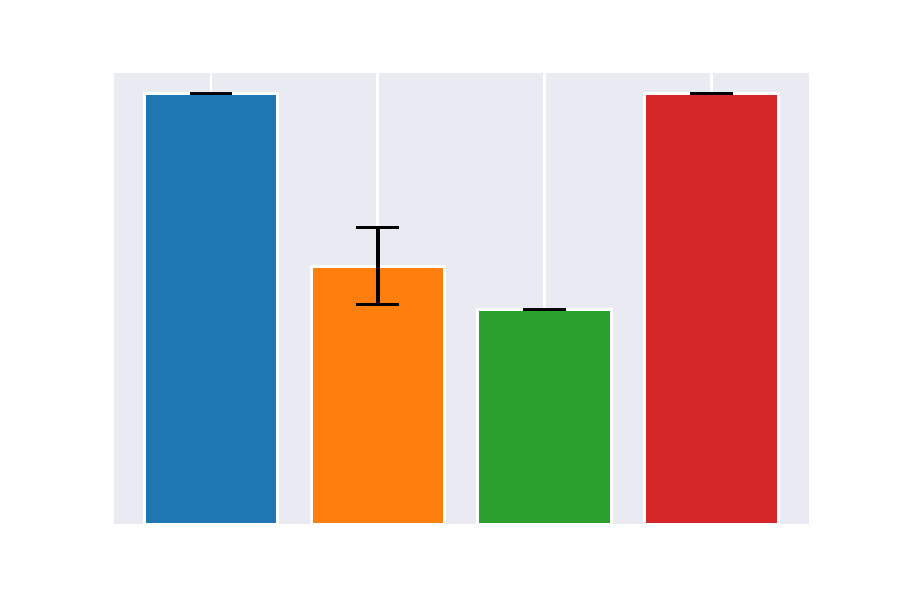
\includegraphics[width=\linewidth]{figs/staghunt_2agent.pdf}
    \caption{2 agents}
    \end{subfigure}
    \begin{subfigure}[b]{.32\linewidth}
    \centering
    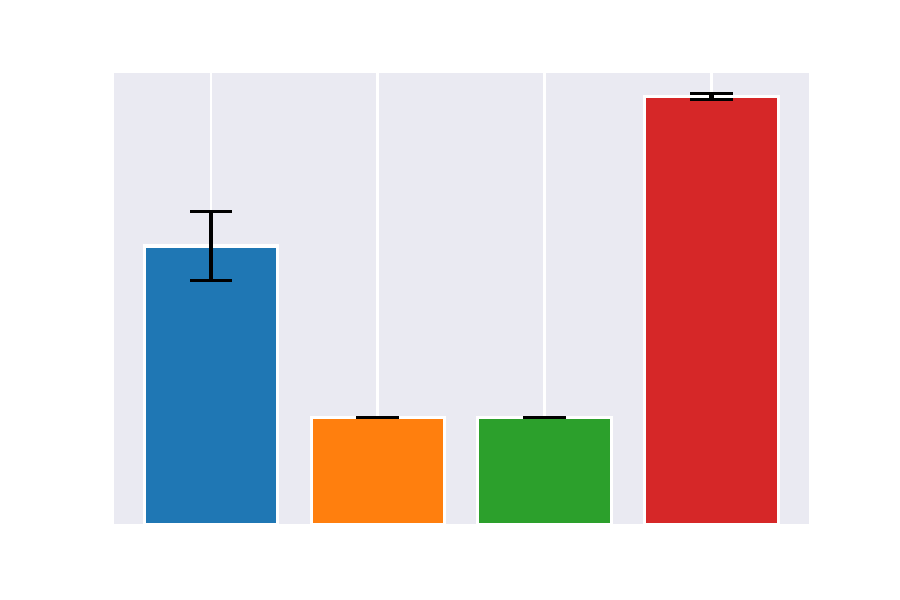
\includegraphics[width=\linewidth]{figs/staghunt_4agent.pdf}
    \caption{4 agents}
    \end{subfigure}
    \begin{subfigure}[b]{.32\linewidth}
    \centering
    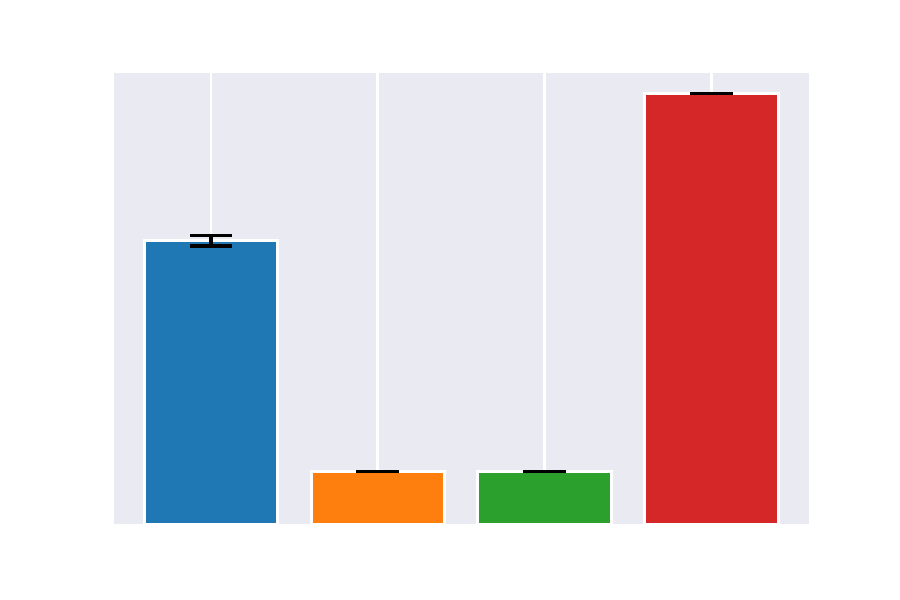
\includegraphics[width=\linewidth]{figs/staghunt_8agent.pdf}
    \caption{8 agents}
    \end{subfigure}
    \caption{Empirical Results for Stag Hunt. As in the case for Prisoner's Dilemma, contracting outperforms both separate and joint training, and always performs at least as well as joint training, significantly outperforming it for high agent counts. As in the Prisoner's Dilemma case in \Cref{fig:matrix}, 5 trials were conducted, algorithms run for 1M timesteps, and the standard error across these trials is reported in the error bars.}
    \label{fig:staghunt}
\end{figure}
\begin{figure}[p]
\centering
\begin{tabular}{|c|c|c|}
\hline 
& C & D \\
\hline 
C & 2,2 & 0,1 \\
\hline 
D & 1,0 & 1,1 \\
\hline
\end{tabular}
\caption{Stag Hunt}
\label{fig:staghuntgame}
\end{figure}